\section{Extraction of the limit on the cross-section}
\label{sec:limitExtraction}
% ---- ---- ---- ---- ---- ---- ---- ---- ---- ---- ---- ---- ---- ---- ---- ---- ---- ---- ---- ---- ---- ---- ----

One strength of this analysis, with the data-driven estimation of the
$W+$jets background, is that we can treat the full mass range,
170-600~\GeV, by the same methods.  We use the ``Higgs Combination''
package \cite{cite:combine} for setting exclusion limits. This package
is a RooStats\cite{cite:roostats}-based statistical analysis toolset
recommended by the CMS Higgs PAG.  Inputs to the limit setter are
RooStats objects representing probability density functions for the
top, diboson, and V+jets backgrounds and signal Monte Carlo (glu-glu
fusion and vector boson fusion), parameterized as described in
Sections~\ref{sec:modelShape} and \ref{sec:wjetsBackground}, and a
dataset for data.

The Higgs mass points are, nominally: 170, 180, 190, 200, 250, 300,
350, 400, 450, 500, 550, and 600~\GeV.  We scale the
signal samples using the cross-section values taken from
\cite{cite:higgsxsecbr}.  Standard Model Higgs cross
sections are described further in Sec.~\ref{sec:MCexpectations}.

To set limits we use the full shape information of the $m_{\ell\nu
  jj}$ distribution.  The four-body mass window is set roughly by the
position and width of the signal distributions for the different Higgs
mass points while trying to maintian adequate sideband for background
determination. The exact values can be seen in
Table~\ref{tab:limitranges}.  All of the distributions are segregated
by lepton flavor, which represents independent channel inputs to the
limit setter.

\begin{table}[tbh]
  \caption{\label{tab:limitranges}Fit ranges and binning for the limit 
    extraction.  The binning was chosen because the combine tool 
    chooses to do binned generation and fits of the ``Asimov'' 
    dataset and we needed to minimize the discrepancy between the 
    binned and unbinned fit results.  In all cases the binning is about 
    10x finer than detector resolution.  Because we have a large amount 
    of background, we have relatively large statistics in most all bins.}
\begin{center}
\begin{tabular}{crrr}
\hline
     & \multicolumn{1}{c}{lower} & \multicolumn{1}{c}{upper} & \\
mass & \multicolumn{1}{c}{limit (GeV)} & \multicolumn{1}{c}{limit (GeV)} & N bins \\
\hline
170 & 165 & 245 & 100 \\
180 & 165 & 245 & 100 \\
190 & 165 & 245 & 100 \\
200 & 165 & 245 & 100 \\
250 & 200 & 400 & 100 \\
300 & 200 & 400 & 100 \\
350 & 250 & 475 & 90 \\
400 & 300 & 600 & 100 \\
450 & 340 & 900 & 140 \\
500 & 340 & 900 & 140 \\
550 & 340 & 900 & 140 \\
600 & 340 & 900 & 140 \\
\hline
\end{tabular}
\end{center}
\end{table}

The systematics described in Section~\ref{sec:systematics} are treated
as follows when being input to the limit setter:
\begin{itemize}
\item The main background systematic uncertainties are total
background shape uncertainty and total background normalization
uncertainty, which are determined by the limit setter when performing
the maximum likelihood fit.
% The
% 1-sigma up- and down-fluctuated background shape inputs to the limit
% setter are shown in Appendix~\ref{app:limitShapes}, along with the
% nominal shapes.  
Both shape and normalization uncertainties are
treated as uncorrelated across all channels, since they are derived
from fits performed on independent sample sets.
\item JES, MET uncertainty, and pileup are considered negligible for
signal and are otherwise subsumed in the normalization/shape
uncertainties for background, so they are omitted from the limit setter
inputs.
\item Uncertainties on the signal deriving from lepton reconstruction
and selection as well as trigger efficiency are treated as uncorrelated
between electron and muon channels.
\item Uncertainties on the signal deriving from parton distribution
functions (Table~\ref{tab:signalPDF}), luminosity, interference, and
theoretical cross-section uncertainty are treated as 100\% correlated
across all channels.
%% Since the PDF and cross-section uncertainties for
%% the gluon fusion process are uniformly worse than those for the vector
%% boson fusion process, the uncertainties for the former are taken as
%% applicable to the summed signal yields.
\item Uncertainties on the signal deriving from the final selection
efficiency are treated as uncorrelated across different channels, but as
correlated between quark-quark and glu-glu signal processes for the same
channel.
\end{itemize}

The limit setter is then set to utilize
the ``asymptotic CL$_{s}$''
\cite{cite:asympcls1,cite:asympcls2} method. 
%The final exclusion limit will be calculated with 
%the ``HybridNew CL$_{s}$'' technique.
The resulting median
expected limit with 1- and 2-sigma error bands are plotted.
The limit plots for all channels combined
(electron and muon)
are shown in
Fig.~\ref{fig:limitsetup:combinedlimit}. 
The background uncertainty is the limiting factor in this analysis.
%%%%%%%%%%%%%%%%%%%%
\begin{figure}[htb] 
  \begin{center}
    \subfigure[]{
%      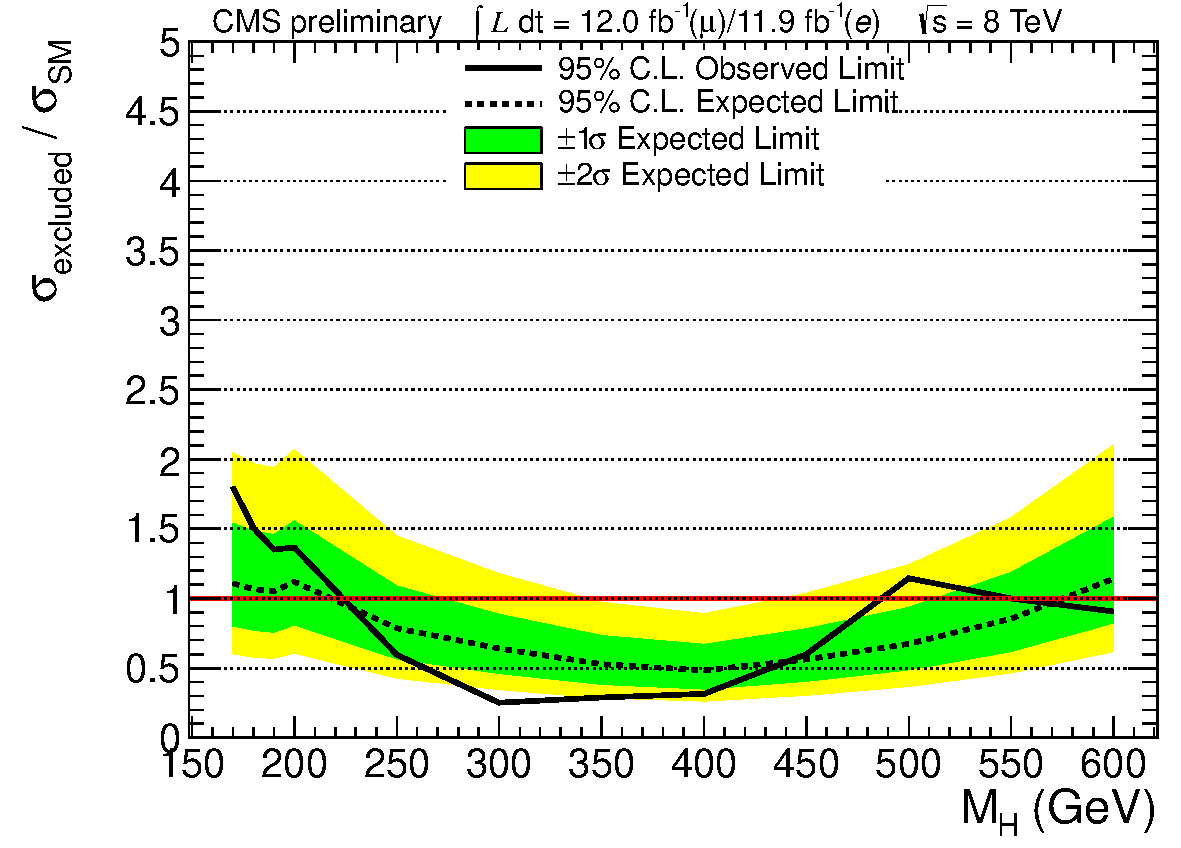
\includegraphics[width=0.48\textwidth]{plots/2012_LIMITS/limit_4chan_fullsyst_asymp.pdf}
      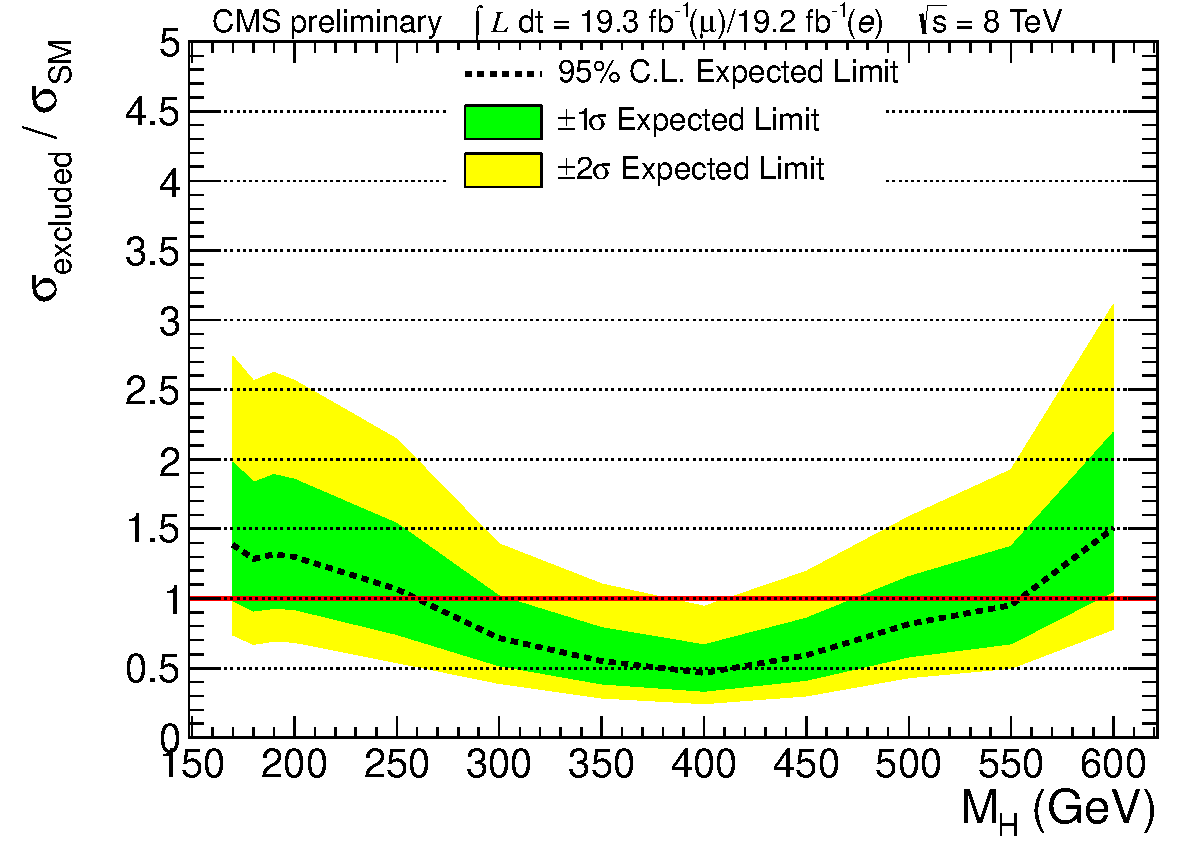
\includegraphics[width=0.48\textwidth]{plots/2012_LIMITS/limit_2chan_fullsyst_asymp.pdf}
%       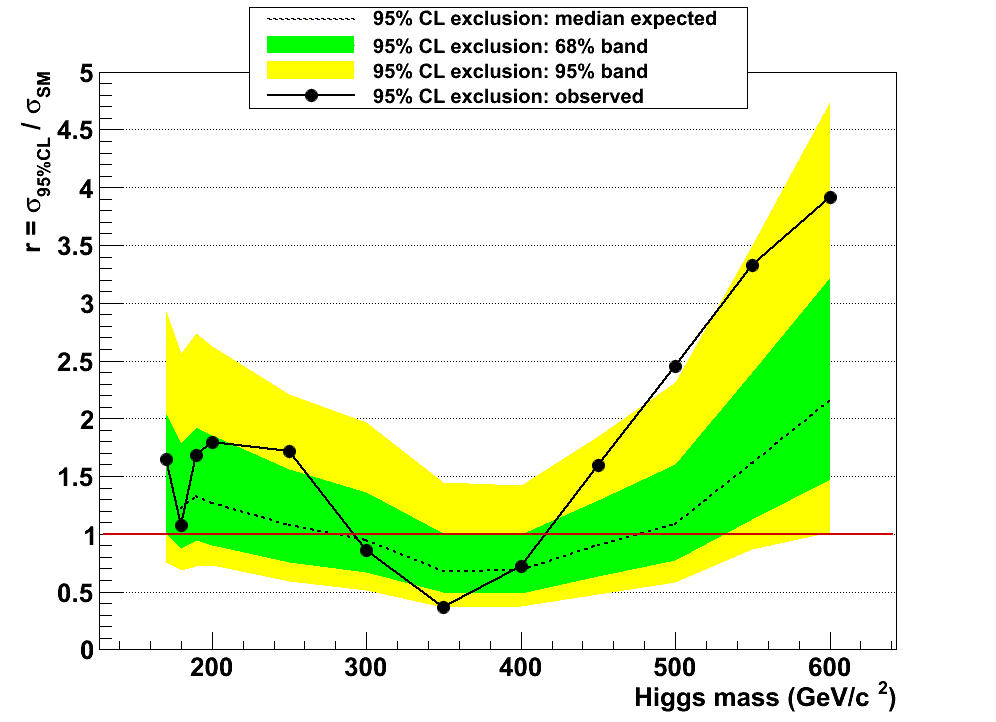
\includegraphics[width=0.6\linewidth]{plots/2012_LIMITS/fullCLs_limits.png}
    }
    \subfigure[]{
      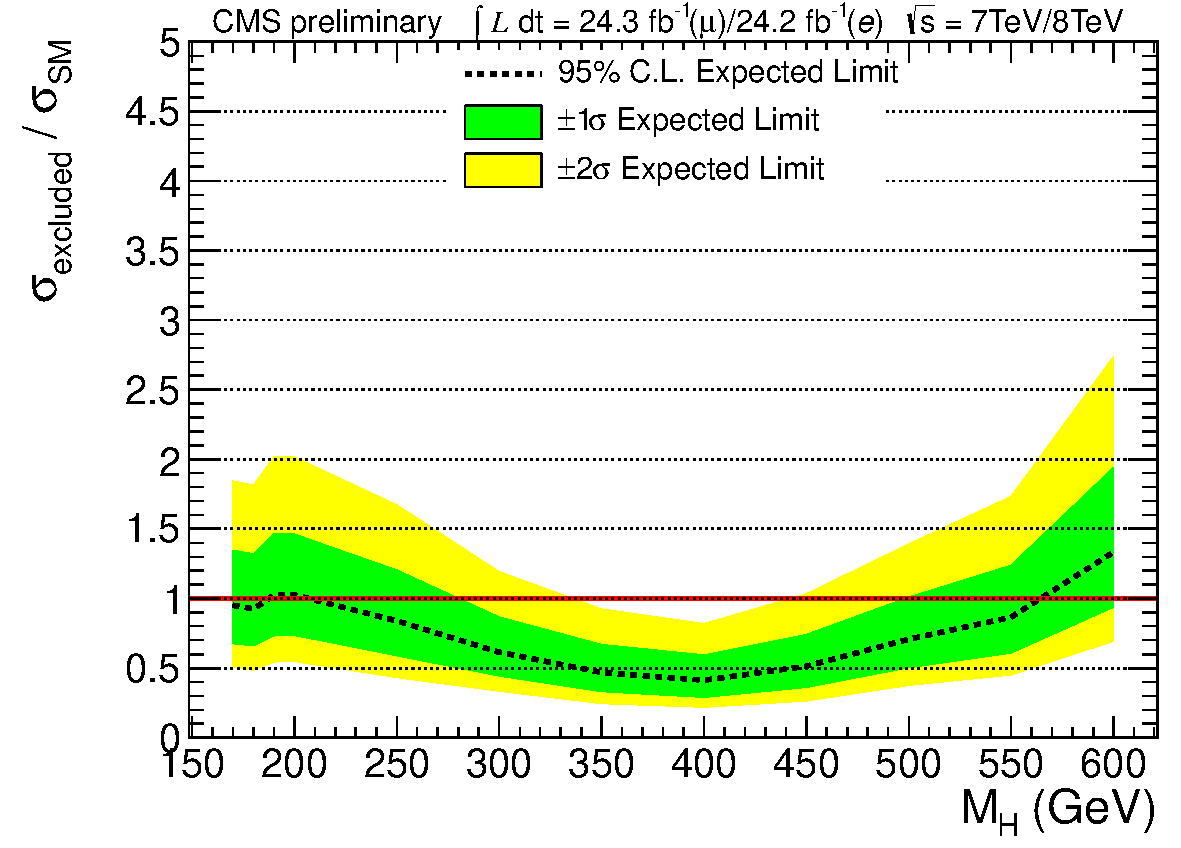
\includegraphics[width=0.48\textwidth]{plots/2012_LIMITS/limit_7and8tevcombined.pdf}
    }
    \\
%%    \subfigure[]{
%%      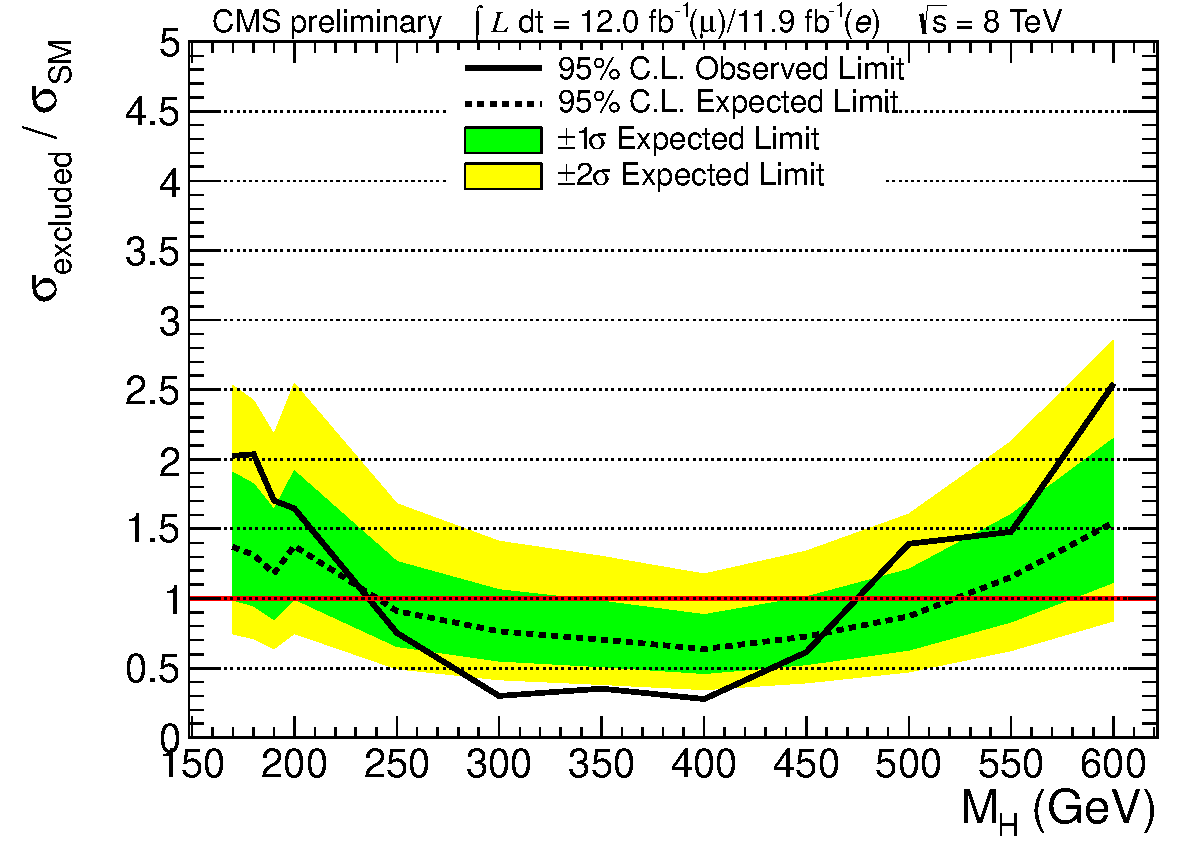
\includegraphics[width=0.48\textwidth]{plots/2012_LIMITS/limit_2jetonly_fullsyst_asymp.pdf}
%%    }
%%     \subfigure[]{
%%       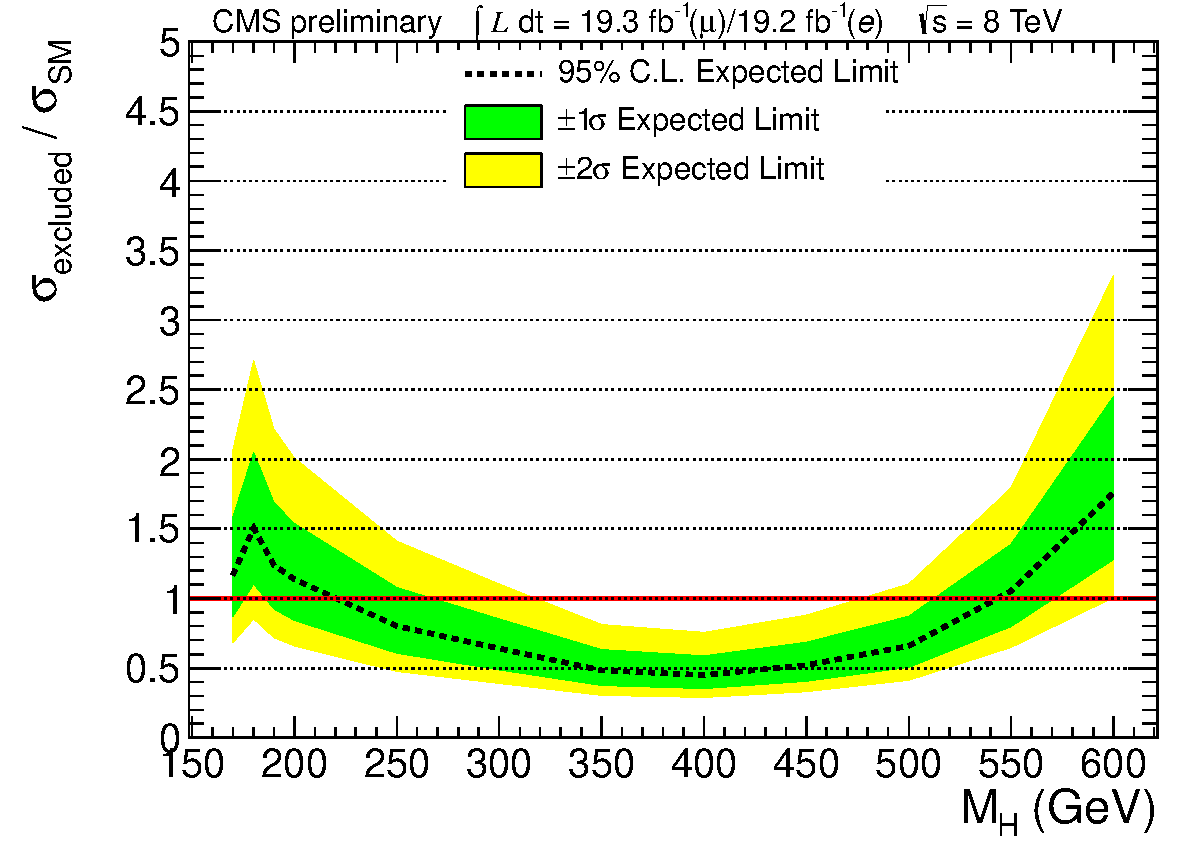
\includegraphics[width=0.48\textwidth]{plots/2012_LIMITS/limit_allchan_nosyst_asymp.pdf}
%%     }
    \caption{The combined Higgs exclusion limit from all channels
      after including all systematic uncertainties (a) from 8~TeV
      data, and (b) for 7 and 8~TeV data combined.
%%      , and (c) for 8~TeV data, statistical uncertainties only (systematic uncertainties removed).
    }
    \label{fig:limitsetup:combinedlimit}
  \end{center}
\end{figure}
%%%%%%%%%%%%%%%%%%%%%%%%%%%%%%%%%%%%%%%%
%%%%%%%%%%%%%%%%%%%%%%%%%%%%%%%%%%%%%%%%
%%%%%%%%%%%%%%%%%%%%%%%%%%%%%%%%%%%%%%%%

Using all channels of 8~TeV data combined, we have sensitivity to
exclude the Standard Model Higgs boson in the mass range
260--550~GeV
to a confidence level of 95\%.
When combined with 7~TeV data~\cite{HIG-12-003}, the sensitive exclusion range expands to
170--190~GeV and 210--560~GeV.
